\documentclass[12pt,a4paper]{article}

% --- Packages -----------------------------------------------------------------
\usepackage{fontspec}
\usepackage{polyglossia}
\setdefaultlanguage{russian}
\setotherlanguage{english}

\setmainfont{Times New Roman}
\setmonofont{Menlo}[Scale=0.85]
\newfontfamily\cyrillicfonttt{Menlo}[Scale=0.85]

\usepackage{amsmath,amssymb,amsthm,mathtools}
\usepackage{geometry}
\geometry{a4paper, left=2.5cm, right=2.0cm, top=2.0cm, bottom=2.0cm}
\usepackage{microtype}
\usepackage{xcolor}
\usepackage{tcolorbox}
\tcbuselibrary{breakable,skins}
\usepackage{enumitem}
\setlist{itemsep=2pt,topsep=4pt}
\usepackage{hyperref}
\hypersetup{colorlinks=true,linkcolor=blue!50!black,urlcolor=blue!50!black}
\usepackage{titlesec}
\titleformat{\section}{\normalfont\Large\bfseries}{\thesection}{0.6em}{}
\titleformat{\subsection}{\normalfont\large\bfseries}{\thesubsection}{0.6em}{}
\usepackage{parskip}
\setlength{\parskip}{6pt}
\setlength{\parindent}{0pt}
\usepackage{booktabs}
\usepackage{array}
\usepackage{multirow}
\usepackage{caption}
\captionsetup{font=small,labelfont=bf}
\usepackage{tikz}
\usetikzlibrary{positioning,arrows.meta,calc}
\usepackage{graphicx}
\graphicspath{{figures/}}
\usepackage{float}

% --- Custom commands ----------------------------------------------------------
\newcommand{\R}{\mathbb{R}}
\newcommand{\E}{\mathbb{E}}
\newcommand{\sign}{\operatorname{sign}}
\newcommand{\argmax}{\operatorname{arg\,max}}
\newcommand{\argmin}{\operatorname{arg\,min}}

\newtcolorbox{intuition}[1][]{
  enhanced,breakable,
  colback=blue!4,colframe=blue!50!black,
  boxrule=0.5pt,arc=2pt,
  title=Интуиция,
  fonttitle=\bfseries,
  #1
}
\newtcolorbox{derivation}[1][]{
  enhanced,breakable,
  colback=gray!5,colframe=gray!50!black,
  boxrule=0.5pt,arc=2pt,
  title=Вывод,
  fonttitle=\bfseries,
  #1
}
\newtcolorbox{example}[1][]{
  enhanced,breakable,
  colback=green!3,colframe=green!40!black,
  boxrule=0.5pt,arc=2pt,
  title=Численный пример,
  fonttitle=\bfseries,
  #1
}
\newtcolorbox{warning}[1][]{
  enhanced,breakable,
  colback=red!3,colframe=red!50!black,
  boxrule=0.5pt,arc=2pt,
  title=Тонкий момент,
  fonttitle=\bfseries,
  #1
}

\title{\textbf{Приложение к ЛР-5}\\\large Градиентный бустинг с нуля:\\интуиция, выводы формул и численные примеры}
\author{Пахомов В.В., группа P3324}
\date{}

\begin{document}
\maketitle

\begin{abstract}
\noindent Это приложение к лабораторной работе подробно разбирает математику градиентного бустинга: что такое слабый учитель, откуда берётся log-loss и сигмоида, почему отрицательный градиент равен $y - \sigma(F)$, как именно «обучение на остатках» эквивалентно градиентному спуску, и зачем нужны learning rate, инициализация log-odds и нормировка One-vs-Rest. Каждая формула из основного отчёта получит здесь подробный вывод, а в конце мы вручную пройдём две итерации бустинга на маленьком примере.
\end{abstract}

\tableofcontents
\vspace{0.5cm}

% ==============================================================================
\section{Идея бустинга: толпа слабых лучше одного сильного}

Пусть мы хотим научиться решать задачу классификации. У нас есть набор простых моделей, каждая из которых работает чуть лучше монеты (например, accuracy $0{,}55$). Такая модель называется \textbf{слабым учителем}. Бустинг говорит:

\begin{quote}
«Возьмём много слабых учителей и сложим их предсказания так, чтобы каждый следующий исправлял ошибки предыдущих. Получится сильный ансамбль.»
\end{quote}

Формально мы строим \textbf{аддитивную модель}:
\[
  F(x) = F_0 + \nu \cdot h_1(x) + \nu \cdot h_2(x) + \cdots + \nu \cdot h_M(x)
       = F_0 + \nu \sum_{m=1}^M h_m(x),
\]
где $h_m$~--- слабые учители (в нашем случае decision stumps), $\nu \in (0, 1]$~--- темп обучения (learning rate), $F_0$~--- начальное значение.

Ключевой вопрос: \emph{как именно выбирать $h_m$, чтобы суммарный ансамбль становился лучше?} Ответ дал Friedman (1999): обучать $h_m$ на отрицательный градиент функции потерь относительно текущего предсказания $F_{m-1}$. Это и есть градиентный бустинг.

\begin{intuition}
Сравните с обычным градиентным спуском: чтобы минимизировать функцию $L(\theta)$ по параметрам $\theta$, мы делаем $\theta \leftarrow \theta - \eta \nabla L$. Идея бустинга~--- делать то же самое, только в \emph{функциональном пространстве}: вместо вектора параметров $\theta$ мы оптимизируем саму функцию $F$. На каждом шаге мы делаем «шаг» в сторону $-\nabla L$, и этот шаг приближается слабым учителем $h_m$.
\end{intuition}

% ==============================================================================
\section{Decision stump: простейший слабый учитель}

\subsection{Что такое stump}

Decision stump~--- это \textbf{дерево решений глубины 1}. Оно выглядит так:

\begin{center}
\begin{tikzpicture}[
  node distance=1.2cm and 2.0cm,
  every node/.style={font=\small},
  root/.style={rectangle, draw, rounded corners, fill=blue!10, minimum width=4cm, minimum height=0.8cm},
  leaf/.style={rectangle, draw, rounded corners, fill=green!10, minimum width=2.8cm, minimum height=0.8cm},
]
  \node[root] (root) {$x_j \le t$ ?};
  \node[leaf, below left=of root] (left) {Лист: $c_L$};
  \node[leaf, below right=of root] (right) {Лист: $c_R$};
  \draw[-Latex] (root) -- node[left] {да} (left);
  \draw[-Latex] (root) -- node[right] {нет} (right);
\end{tikzpicture}
\end{center}

Формально:
\[
  h(x) = c_L \cdot [x_j \le t] + c_R \cdot [x_j > t],
\]
где квадратные скобки $[\cdot]$~--- индикатор условия (1 если истинно, 0 иначе), $j$~--- индекс выбранного признака, $t$~--- порог, $c_L, c_R$~--- значения для левого и правого листьев.

\begin{intuition}
Это просто if-else: если значение $j$-го признака $\le t$, выдаём $c_L$, иначе $c_R$. Никакой магии. В нашем коде:
\begin{quote}\small\ttfamily
return np.where(X[:, feature\_idx] <= threshold, left\_value, right\_value)
\end{quote}
\end{intuition}

\subsection{Как обучается stump на остатках}

В градиентном бустинге каждый stump обучается \emph{не на исходных метках} $y$, а на \textbf{остатках} $r_i$ (negative gradient текущего ансамбля). Мы хотим, чтобы $h(x_i) \approx r_i$, то есть минимизировать
\[
  \sum_{i=1}^n \bigl(r_i - h(x_i)\bigr)^2.
\]

\textbf{Вопрос:} при фиксированных $j$ и $t$, какие $c_L$ и $c_R$ минимизируют эту сумму?

\begin{derivation}
Разобьём объекты на $S_L = \{i : x_{ij} \le t\}$ и $S_R = \{i : x_{ij} > t\}$. Сумма раскладывается:
\[
  \sum_{i \in S_L} (r_i - c_L)^2 + \sum_{i \in S_R} (r_i - c_R)^2.
\]

Это две независимые квадратичные функции. Производная по $c_L$:
\[
  \frac{\partial}{\partial c_L}\sum_{i \in S_L}(r_i - c_L)^2 = -2\sum_{i \in S_L}(r_i - c_L) = 0
  \;\Longrightarrow\;
  c_L^* = \frac{1}{|S_L|}\sum_{i \in S_L} r_i.
\]

Аналогично $c_R^* = \frac{1}{|S_R|}\sum_{i \in S_R} r_i$. То есть оптимальное значение листа~--- это \textbf{среднее остатков} в нём. Это базовый факт линейной алгебры: $\bar{x}$ минимизирует $\sum(x_i - c)^2$.
\end{derivation}

\textbf{Поиск $(j, t)$.} Перебираем все признаки $j \in \{1, \ldots, d\}$ (в нашем коде~--- случайную подвыборку из 24 признаков из 561). Для каждого $j$ перебираем кандидаты на порог $t$ (50 квантилей колонки $X_{:,j}$). Для каждой пары $(j, t)$ считаем $c_L^*, c_R^*$ и итоговый loss $\sum(r_i - h(x_i))^2$. Выбираем $(j, t, c_L, c_R)$ с минимальным loss'ом.

\begin{figure}[H]
  \centering
  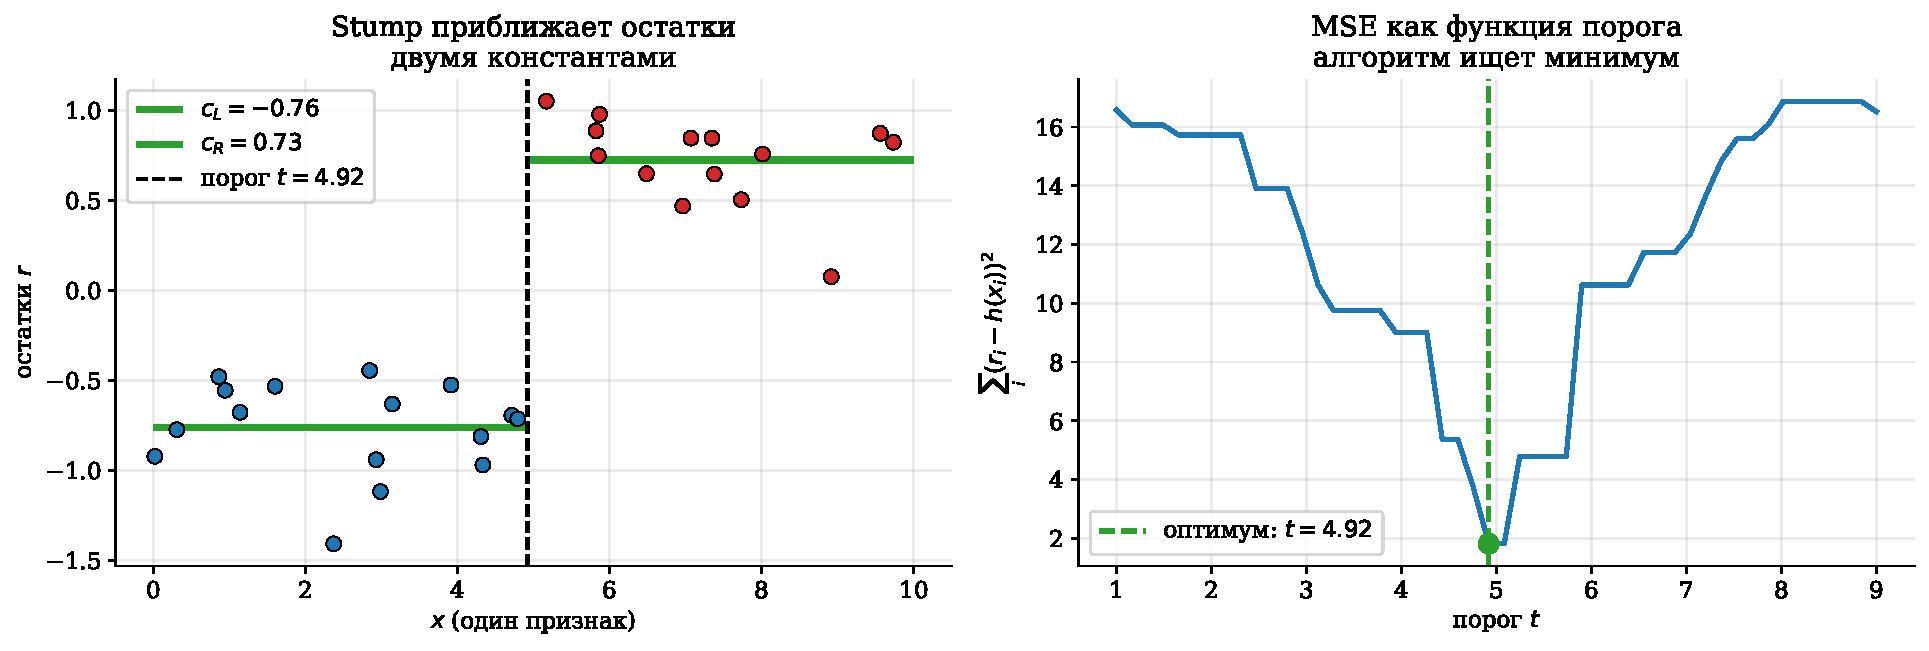
\includegraphics[width=1.0\linewidth]{decision_stump.pdf}
  \caption{Декомпозиция работы decision stump на одномерном примере. Слева: точки~--- остатки $r_i$, зелёные горизонтальные линии~--- константы $c_L$ и $c_R$, на которые stump «приближает» $r$ слева и справа от порога. Справа: MSE как функция порога~--- алгоритм перебирает все $t$ из набора квантилей и берёт минимум.}
\end{figure}

\subsection{Почему квантили вместо всех уникальных значений}

В колонке может быть 7000 уникальных значений. Перебирать все 7000 порогов = считать loss 7000 раз на каждом признаке = очень медленно. Квантили дают 50 «равномерных» порогов по распределению признака~--- этого достаточно для разумного разбиения, и работает в $7000/50 = 140$ раз быстрее.

\begin{warning}
Квантили~--- это эвристика. Теоретически оптимальный порог может оказаться между квантильными. На практике потеря в качестве пренебрежима, а ускорение огромно.
\end{warning}

% ==============================================================================
\section{Log-loss и сигмоида: вероятностный смысл}

\subsection{От задачи классификации к вероятности}

Бинарная классификация: $y \in \{0, 1\}$. Модель выдаёт некий \emph{сырой выход} $F(x) \in \R$ (произвольное число, может быть отрицательным, может быть огромным). Чтобы из $F$ получить вероятность класса 1, нужна функция, переводящая $\R \to [0, 1]$.

Самый естественный выбор~--- \textbf{сигмоида}:
\[
  \sigma(F) = \frac{1}{1 + e^{-F}}.
\]

\subsection{Откуда берётся именно сигмоида}

\begin{derivation}
Предположим, что $\log\bigl(\Pr(y=1 \mid x) / \Pr(y=0 \mid x)\bigr) = F(x)$. Это называется \emph{log-odds} (логарифм отношения шансов). Обозначим $p = \Pr(y=1)$. Тогда:
\[
  \log\frac{p}{1-p} = F \;\Longrightarrow\; \frac{p}{1-p} = e^F \;\Longrightarrow\; p = (1-p)e^F.
\]
Раскрываем: $p = e^F - p e^F$, откуда $p(1 + e^F) = e^F$, или
\[
  p = \frac{e^F}{1 + e^F} = \frac{1}{e^{-F} + 1} = \sigma(F).
\]
\end{derivation}

То есть сигмоида~--- это просто обратная функция к log-odds. Использование $\sigma$ означает, что мы моделируем log-odds линейной (или, для бустинга, аддитивной) функцией признаков.

\begin{figure}[H]
  \centering
  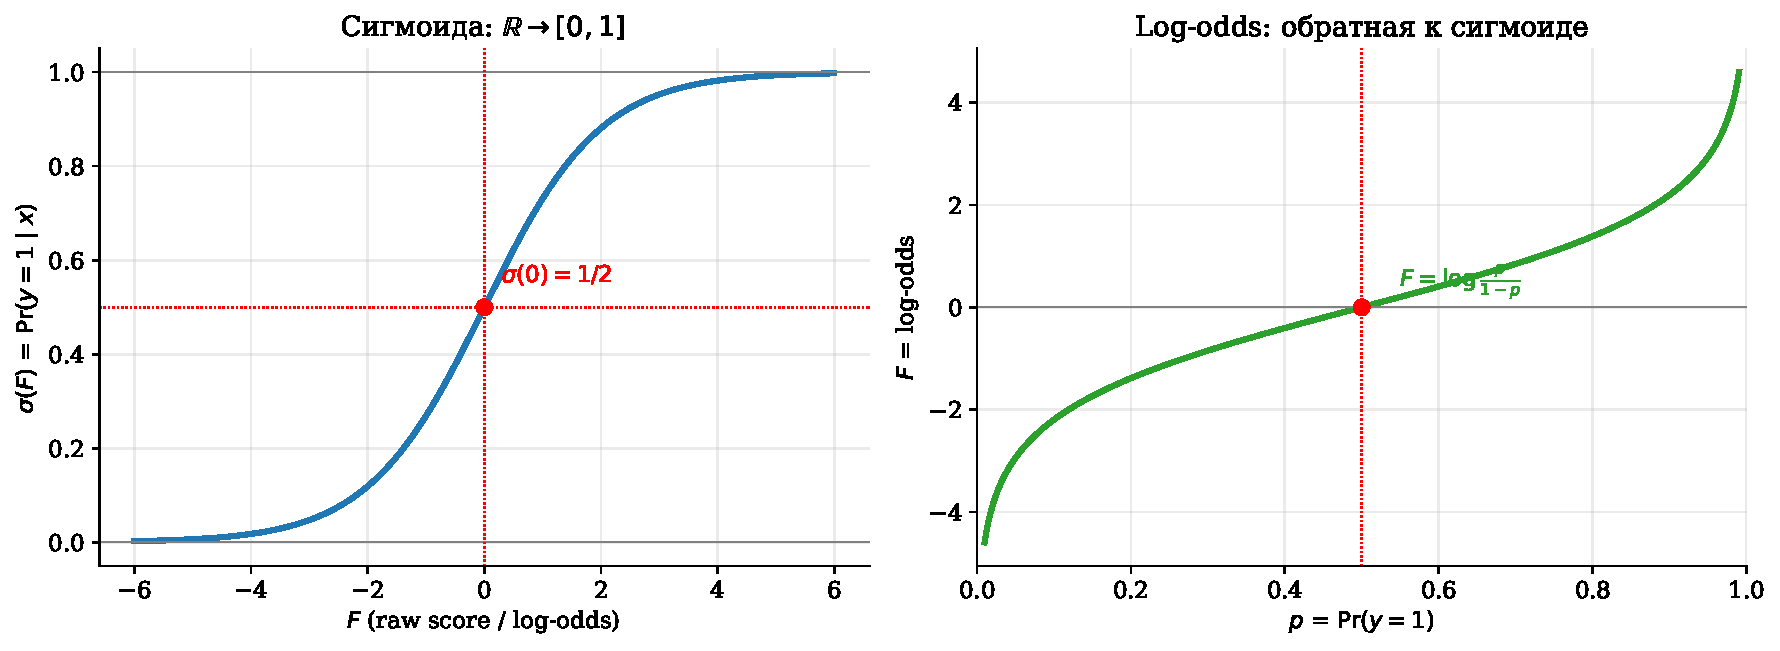
\includegraphics[width=1.0\linewidth]{sigmoid_logodds.pdf}
  \caption{Слева: сигмоида $\sigma(F)$ переводит произвольное вещественное $F$ в вероятность $[0, 1]$. В точке $F = 0$ вероятность ровно $1/2$. Справа: обратная функция~--- log-odds $\log(p/(1-p))$. Бустинг моделирует $F(x)$ (log-odds) аддитивно, и финальная вероятность получается прогоном через сигмоиду.}
\end{figure}

\subsection{Свойства $\sigma$}

\begin{itemize}
  \item $\sigma(0) = 1/2$, $\sigma(+\infty) = 1$, $\sigma(-\infty) = 0$.
  \item $\sigma(-F) = 1 - \sigma(F)$ (симметрия).
  \item \textbf{Производная:} $\sigma'(F) = \sigma(F)\bigl(1 - \sigma(F)\bigr)$.
\end{itemize}

\begin{derivation}
Производная сигмоиды (понадобится при выводе остатков):
\[
  \sigma'(F) = \frac{d}{dF}\frac{1}{1+e^{-F}}
  = \frac{e^{-F}}{(1+e^{-F})^2}
  = \frac{1}{1+e^{-F}} \cdot \frac{e^{-F}}{1+e^{-F}}
  = \sigma(F) \cdot (1 - \sigma(F)).
\]
\end{derivation}

\subsection{Log-loss как максимальное правдоподобие}

Метка $y \in \{0, 1\}$, модель говорит $\Pr(y = 1 \mid x) = \sigma(F(x)) = p$. Тогда $\Pr(y = 0 \mid x) = 1 - p$. \textbf{Правдоподобие} одной точки:
\[
  P(y \mid x) = p^y (1-p)^{1-y} =
  \begin{cases}
    p, & y = 1\\
    1-p, & y = 0
  \end{cases}
\]

Хотим максимизировать $P(y \mid x)$ по параметрам. Удобнее работать с логарифмом:
\[
  \log P(y \mid x) = y \log p + (1-y)\log(1-p).
\]

Это и есть формула \textbf{log-likelihood}. Максимизация $\log P$ эквивалентна минимизации $-\log P$, что и есть log-loss:
\[
  \boxed{
  L(y, F) = -\bigl[y \log \sigma(F) + (1-y)\log(1 - \sigma(F))\bigr]
  }
\]

\begin{intuition}
Если $y = 1$, $L = -\log \sigma(F)$. Чтобы $L$ был маленький, нужно $\sigma(F) \to 1$, то есть $F \to +\infty$.

Если $y = 0$, $L = -\log(1 - \sigma(F)) = -\log \sigma(-F)$. Нужно $\sigma(-F) \to 1$, то есть $F \to -\infty$.

То есть log-loss «толкает» $F$ в сторону $+\infty$ для $y = 1$ и $-\infty$ для $y = 0$, но \emph{асимптотически}~--- логарифм растёт медленно, поэтому уверенные правильные ответы поощряются слабо, а уверенные \emph{неправильные} штрафуются жёстко.
\end{intuition}

% ==============================================================================
\section{Главный вывод: residuals = $y - \sigma(F)$}

Это самая важная формула во всём бустинге. Её надо понять.

\subsection{Что мы хотим вычислить}

Мы оптимизируем $L(y, F)$ \emph{по $F$} (рассматриваем $F$ как переменную, как будто это параметр). На каждой итерации хотим найти направление, куда сдвинуть $F$, чтобы $L$ уменьшилось. Это направление~--- \emph{отрицательный градиент}:
\[
  r = -\frac{\partial L}{\partial F}.
\]

\subsection{Вывод}

\begin{derivation}
Раскроем $L$:
\[
  L = -y \log \sigma(F) - (1-y)\log(1 - \sigma(F)).
\]

Производная по $F$:
\[
  \frac{\partial L}{\partial F}
  = -y \cdot \frac{\sigma'(F)}{\sigma(F)} - (1-y) \cdot \frac{-\sigma'(F)}{1 - \sigma(F)}.
\]

Используем $\sigma'(F) = \sigma(F)(1 - \sigma(F))$:
\[
  = -y \cdot \frac{\sigma(F)(1-\sigma(F))}{\sigma(F)} + (1-y) \cdot \frac{\sigma(F)(1-\sigma(F))}{1-\sigma(F)}
  = -y(1 - \sigma(F)) + (1-y)\sigma(F).
\]

Раскрываем:
\[
  = -y + y\sigma(F) + \sigma(F) - y\sigma(F) = \sigma(F) - y.
\]

\textbf{Итого:}
\[
  \frac{\partial L}{\partial F} = \sigma(F) - y,
  \qquad
  -\frac{\partial L}{\partial F} = y - \sigma(F).
\]
\end{derivation}

То есть \textbf{отрицательный градиент log-loss равен $(y - \sigma(F))$}, это и есть наши «остатки» (residuals).

\subsection{Интуиция}

\begin{intuition}
$y - \sigma(F)$~--- это \textbf{ошибка предсказания вероятности}:
\begin{itemize}
  \item Если $y = 1$ и $\sigma(F) = 0{,}3$ (мы говорим «вероятность Target $30\%$»), то $r = 1 - 0{,}3 = 0{,}7$. Большое положительное значение~--- надо сильно сдвинуть $F$ \emph{вверх}.
  \item Если $y = 1$ и $\sigma(F) = 0{,}99$ (мы почти уверены), то $r = 0{,}01$. Маленькое~--- сдвиг почти не нужен.
  \item Если $y = 0$ и $\sigma(F) = 0{,}8$ (мы ошибаемся, говорим «Target»), то $r = 0 - 0{,}8 = -0{,}8$. Большое отрицательное~--- сдвинуть $F$ \emph{вниз}.
\end{itemize}

Это в точности то, чего мы хотим. Бустинг говорит: «следующее дерево, угадай-ка $r_i$ для каждого объекта; куда мы тебя сдвинем, туда и пойдём».
\end{intuition}

\begin{figure}[H]
  \centering
  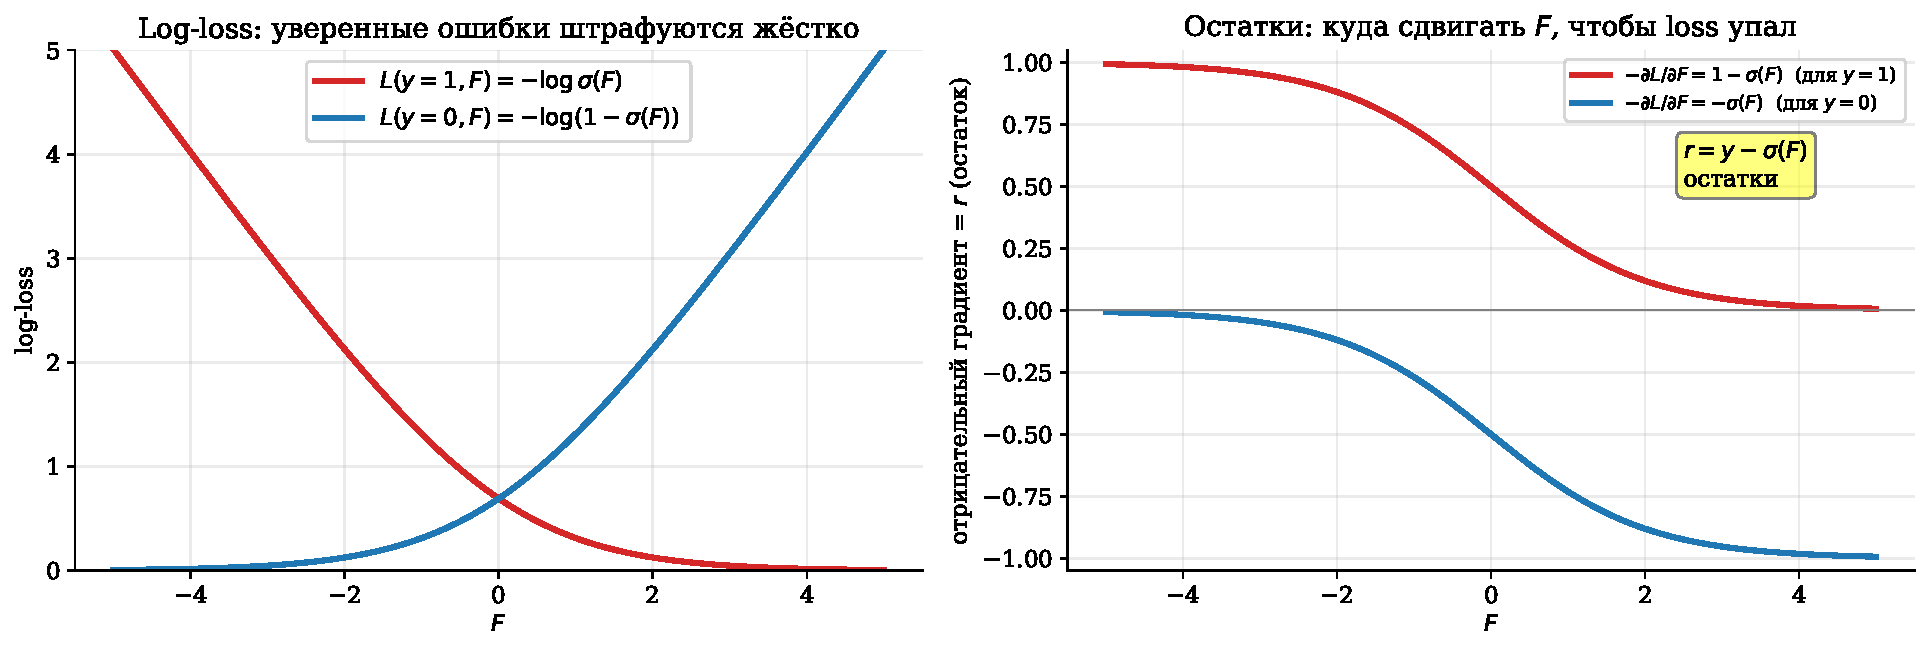
\includegraphics[width=0.92\linewidth]{logloss_and_gradient.pdf}
  \caption{Слева: log-loss как функция от $F$. Для $y = 1$ (красная) минимум при $F \to +\infty$, и наоборот для $y = 0$. Уверенно неверный ответ штрафуется почти линейно (огромный loss). Справа: отрицательный градиент $-\partial L/\partial F$~--- это и есть остаток $r = y - \sigma(F)$. Знак показывает, в какую сторону сдвинуть $F$, чтобы loss упал; модуль~--- насколько сильно.}
\end{figure}

\begin{figure}[H]
  \centering
  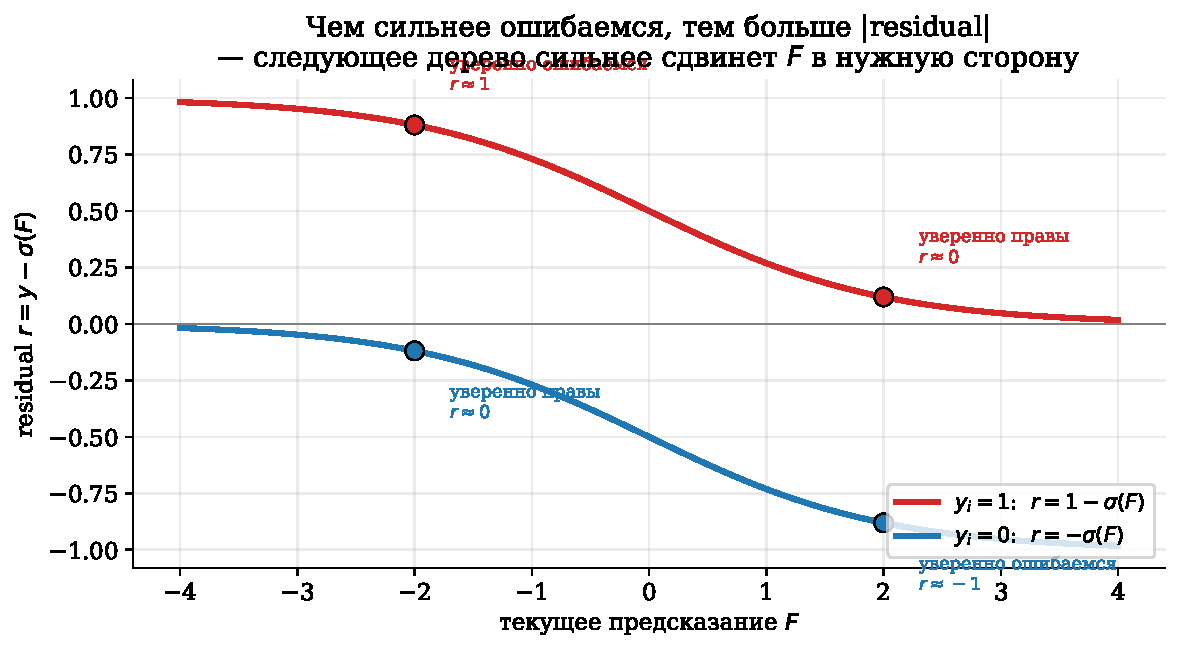
\includegraphics[width=0.85\linewidth]{residuals_field.pdf}
  \caption{Residuals для четырёх типичных ситуаций. Когда модель уверенно ошибается, $|r| \to 1$ и следующее дерево получает сильный сигнал «двигайся сюда». Когда модель уверенно права, $|r| \to 0$ и следующее дерево почти не трогает этот объект. Это автоматически концентрирует усилия на трудных примерах~--- ключевая особенность бустинга.}
\end{figure}

\subsection{Связь с MSE-боустингом}

Для регрессии с MSE loss $L = (y - F)^2/2$ имеем $\partial L/\partial F = -(y - F)$, то есть $r = y - F$. В этом случае «обучить дерево на остатках» $r$ означает буквально приближать $y - F$. Для классификации с log-loss идея та же, только остатки имеют чуть другой вид: $r = y - \sigma(F)$, где $\sigma$ переводит $F$ в вероятность.

% ==============================================================================
\section{Стартовое значение $F_0 = \log(p/(1-p))$}

\subsection{Зачем нужно $F_0$}

Если стартовать с $F_0 = 0$, то начальная вероятность $\sigma(0) = 0{,}5$. Это означает: «без всякой информации модель думает, что класс Target с вероятностью 50\%». Но в нашей задаче P300 \emph{априори} класс 1 составляет 17\%! Стартовать с $0{,}5$~--- значит первые несколько деревьев потратятся только на «выправление смещения», а не на изучение паттернов.

\subsection{Оптимальное $F_0$}

Хотим выбрать константу $F_0$, минимизирующую log-loss на всей выборке:
\[
  F_0 = \argmin_F \sum_i L(y_i, F).
\]

\begin{derivation}
Производная по $F$:
\[
  \sum_i \frac{\partial L_i}{\partial F} = \sum_i \bigl(\sigma(F) - y_i\bigr) = n\sigma(F) - \sum_i y_i = 0.
\]
Отсюда $\sigma(F) = \bar{y} = p$, где $p$~--- доля положительных в выборке. Применяя обратную функцию (это и есть log-odds):
\[
  F_0 = \sigma^{-1}(p) = \log \frac{p}{1 - p}.
\]
\end{derivation}

\textbf{Пример.} У нас 17\% Target. Тогда $p = 0{,}17$, и
\[
  F_0 = \log\frac{0{,}17}{0{,}83} \approx \log 0{,}205 \approx -1{,}59.
\]

Это значит: до обучения каких-либо деревьев модель считает, что log-odds быть Target равны $-1{,}59$, то есть Target менее вероятен в $e^{1{,}59} \approx 4{,}9$ раз. И это \emph{соответствует} истинной пропорции $83/17 \approx 4{,}9$.

\begin{intuition}
$F_0 = \log(p/(1-p))$~--- это оптимальный «постоянный» классификатор. Бустинг говорит: «Я начну с лучшего, что можно сделать без информации о $x$. Дальше деревья будут добавлять информацию о $x$.»
\end{intuition}

% ==============================================================================
\section{Полный алгоритм бинарного бустинга}

\textbf{Вход:} обучающая выборка $(x_i, y_i)$, $y_i \in \{0, 1\}$, $i = 1, \ldots, n$. Гиперпараметры: число деревьев $M$, темп $\nu$, размер подвыборки признаков $k$.

\begin{enumerate}
  \item Инициализация:
    $\displaystyle F_0 = \log\frac{p}{1-p}$, где $p = \frac{1}{n}\sum_i y_i$.
    Вектор предсказаний $F = (F_0, F_0, \ldots, F_0)$.
  \item Для $m = 1, 2, \ldots, M$:
    \begin{enumerate}
      \item Вычислить вероятности: $p_i = \sigma(F_i)$ для всех $i$.
      \item Вычислить остатки: $r_i = y_i - p_i$.
      \item Выбрать случайную подвыборку признаков $J_m \subset \{1, \ldots, d\}$, $|J_m| = k$.
      \item Обучить stump $h_m$ на $(X, r)$, используя только признаки $J_m$. Получаем $(j_m, t_m, c_L^{(m)}, c_R^{(m)})$.
      \item Обновить $F_i \leftarrow F_i + \nu \cdot h_m(x_i)$ для всех $i$.
    \end{enumerate}
  \item Возврат: ансамбль $\{F_0, h_1, h_2, \ldots, h_M, \nu\}$.
\end{enumerate}

\textbf{Предсказание для нового $x$:}
\[
  F(x) = F_0 + \nu \sum_{m=1}^M h_m(x), \quad
  \hat{p}(x) = \sigma(F(x)), \quad
  \hat{y}(x) = [\hat{p}(x) > 0{,}5].
\]

\subsection{Учим ли мы веса листьев именно так}

\begin{warning}
В строгом ($\textbf{«классическом»}$) Friedman-бустинге для log-loss значения листьев находятся \emph{специальной оптимизацией}, а не просто как среднее остатков. Формула:
\[
  c_{\text{лист}} = \frac{\sum_{i \in S} r_i}{\sum_{i \in S} p_i (1 - p_i)}.
\]

Это поправка на «кривизну» log-loss в точке~--- по сути, шаг Ньютона вместо градиентного шага. Наша реализация использует упрощённую версию (просто среднее $r_i$), что эквивалентно градиентному спуску по $L$ через приближение MSE. Качество на HAR от этого почти не страдает; настоящие движки типа XGBoost используют Newton-вариант.
\end{warning}

\subsection{Зачем нужен learning rate $\nu$}

Без $\nu$ (то есть $\nu = 1$) бустинг сделал бы большой шаг по градиенту на каждой итерации. Это рискованно: переборщили~--- модель «перепрыгивает» через оптимум.

$\nu = 0{,}1$ в коде означает: «доверяй каждому дереву только на 10\%». Деревьев нужно больше (то есть $M$ растёт), зато сходимость гладкая и обобщение лучше.

\begin{intuition}
Подобно learning rate в обычном GD: мелкий шаг = больше итераций, лучшее обобщение; крупный шаг = быстрее, но рискуем «прыгать» и переобучаться.

Эмпирический закон: при уменьшении $\nu$ в 10 раз нужно увеличить $M$ примерно в 10 раз, чтобы сохранить сходимость.
\end{intuition}

\begin{figure}[H]
  \centering
  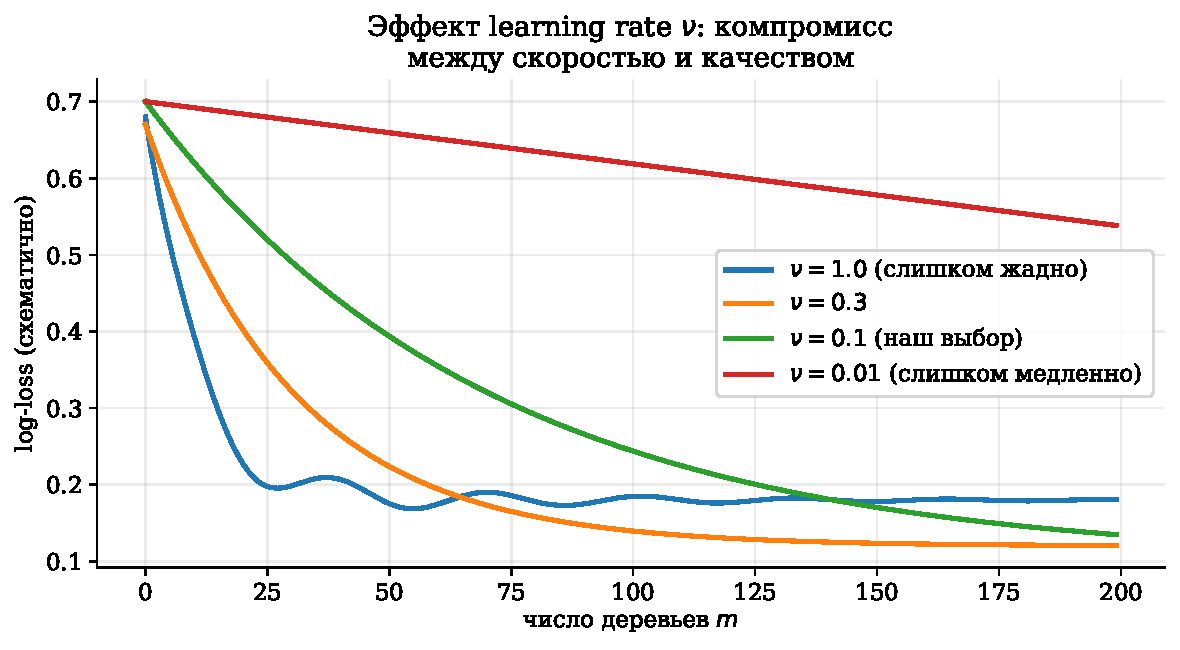
\includegraphics[width=0.85\linewidth]{learning_rate.pdf}
  \caption{Эффект $\nu$ на сходимость (схематично). При $\nu = 1$ модель резко падает в начале, но потом «прыгает» и не достигает минимума. При $\nu = 0{,}01$ слишком медленно. $\nu = 0{,}1$ (наш выбор)~--- разумный компромисс: 100 деревьев успевают сойтись, но без перепрыгивания.}
\end{figure}

% ==============================================================================
\section{Численный пример: 2 итерации бустинга руками}

Возьмём игрушечную бинарную задачу:
\begin{center}
\begin{tabular}{cccc}
\toprule
$i$ & $x_i$ (одномерный) & $y_i$\\
\midrule
1 & $1$ & $0$\\
2 & $2$ & $0$\\
3 & $3$ & $1$\\
4 & $4$ & $1$\\
\bottomrule
\end{tabular}
\end{center}

Гиперпараметры: $\nu = 0{,}5$ (для наглядности), $M = 2$, stump перебирает порог из $\{1{,}5;\; 2{,}5;\; 3{,}5\}$.

\textbf{Шаг 0: Инициализация.}
$p = 2/4 = 0{,}5$, $F_0 = \log(0{,}5/0{,}5) = 0$. То есть $F = (0, 0, 0, 0)$, $\sigma(F) = (0{,}5;\; 0{,}5;\; 0{,}5;\; 0{,}5)$.

\textbf{Шаг 1: Первое дерево.}

Остатки: $r_i = y_i - \sigma(F_i) = (0-0{,}5;\; 0-0{,}5;\; 1-0{,}5;\; 1-0{,}5) = (-0{,}5;\; -0{,}5;\; 0{,}5;\; 0{,}5)$.

Перебираем пороги:
\begin{itemize}
  \item $t = 1{,}5$: $S_L = \{1\}$, $c_L = -0{,}5$; $S_R = \{2,3,4\}$, $c_R = (-0{,}5 + 0{,}5 + 0{,}5)/3 = 0{,}167$.\\
    Loss: $(-0{,}5 - (-0{,}5))^2 + 3 \cdot (\text{среднее отклонение в } S_R)^2 = 0 + (\text{var}(S_R) \cdot 3)$.\\
    Подсчёт: $r_{S_R} = (-0{,}5;\; 0{,}5;\; 0{,}5)$, отклонения от $0{,}167$: $(-0{,}667;\; 0{,}333;\; 0{,}333)$, квадраты сумма $= 0{,}667$.\\
    \textbf{Loss} $= 0 + 0{,}667 = 0{,}667$.
  \item $t = 2{,}5$: $S_L = \{1, 2\}$, $c_L = -0{,}5$; $S_R = \{3, 4\}$, $c_R = 0{,}5$.\\
    Все объекты совпадают со средним $\Rightarrow$ \textbf{Loss} $= 0$. \emph{Идеальное разбиение.}
  \item $t = 3{,}5$: $S_L = \{1,2,3\}$, $c_L = -0{,}167$; $S_R = \{4\}$, $c_R = 0{,}5$. Loss $= 0{,}667$.
\end{itemize}

Выбираем $t = 2{,}5$, $c_L = -0{,}5$, $c_R = 0{,}5$. Это и есть наш первый stump $h_1$.

Обновление: $F_i \leftarrow F_i + 0{,}5 \cdot h_1(x_i)$.
\[
  h_1 = (-0{,}5;\; -0{,}5;\; 0{,}5;\; 0{,}5), \quad
  F = (0;\; 0;\; 0;\; 0) + 0{,}5 \cdot (-0{,}5;\; -0{,}5;\; 0{,}5;\; 0{,}5)
  = (-0{,}25;\; -0{,}25;\; 0{,}25;\; 0{,}25).
\]

Вероятности: $\sigma(-0{,}25) \approx 0{,}438$, $\sigma(0{,}25) \approx 0{,}562$. То есть уже сдвинули в правильную сторону.

\textbf{Шаг 2: Второе дерево.}

Остатки: $r = y - \sigma(F) = (0 - 0{,}438;\; 0 - 0{,}438;\; 1 - 0{,}562;\; 1 - 0{,}562) = (-0{,}438;\; -0{,}438;\; 0{,}438;\; 0{,}438)$.

Аналогично, лучший порог $t = 2{,}5$, $c_L = -0{,}438$, $c_R = 0{,}438$. (Структура задачи прежняя, только остатки уменьшились по модулю.)

Обновление: $F = (-0{,}25;\; -0{,}25;\; 0{,}25;\; 0{,}25) + 0{,}5 \cdot (-0{,}438;\; -0{,}438;\; 0{,}438;\; 0{,}438)$
\[
  = (-0{,}469;\; -0{,}469;\; 0{,}469;\; 0{,}469).
\]

Вероятности: $\sigma(-0{,}469) \approx 0{,}385$, $\sigma(0{,}469) \approx 0{,}615$. Двигаемся к правильным $0$ и $1$, но \emph{медленно}~--- именно из-за $\nu = 0{,}5$.

\begin{example}
Если бы взяли $\nu = 1$, после первой итерации $F = (-0{,}5; -0{,}5; 0{,}5; 0{,}5)$, $\sigma(F) = (0{,}378; 0{,}378; 0{,}622; 0{,}622)$. Та же сторона, но дальше от центра. На 2-й итерации residuals были бы тоже меньше, но менее сжаты~--- быстрее сходились бы в итоге.

После, скажем, 100 итераций с $\nu = 0{,}1$ модель достигнет вероятностей вроде $\sigma(F_3) \approx 0{,}99$ для классов Target, $\sigma(F_1) \approx 0{,}01$ для NonTarget~--- то есть почти уверенные предсказания. Каждый stump добавляет крохотную поправку, и в сумме получается мощный классификатор.
\end{example}

\begin{figure}[H]
  \centering
  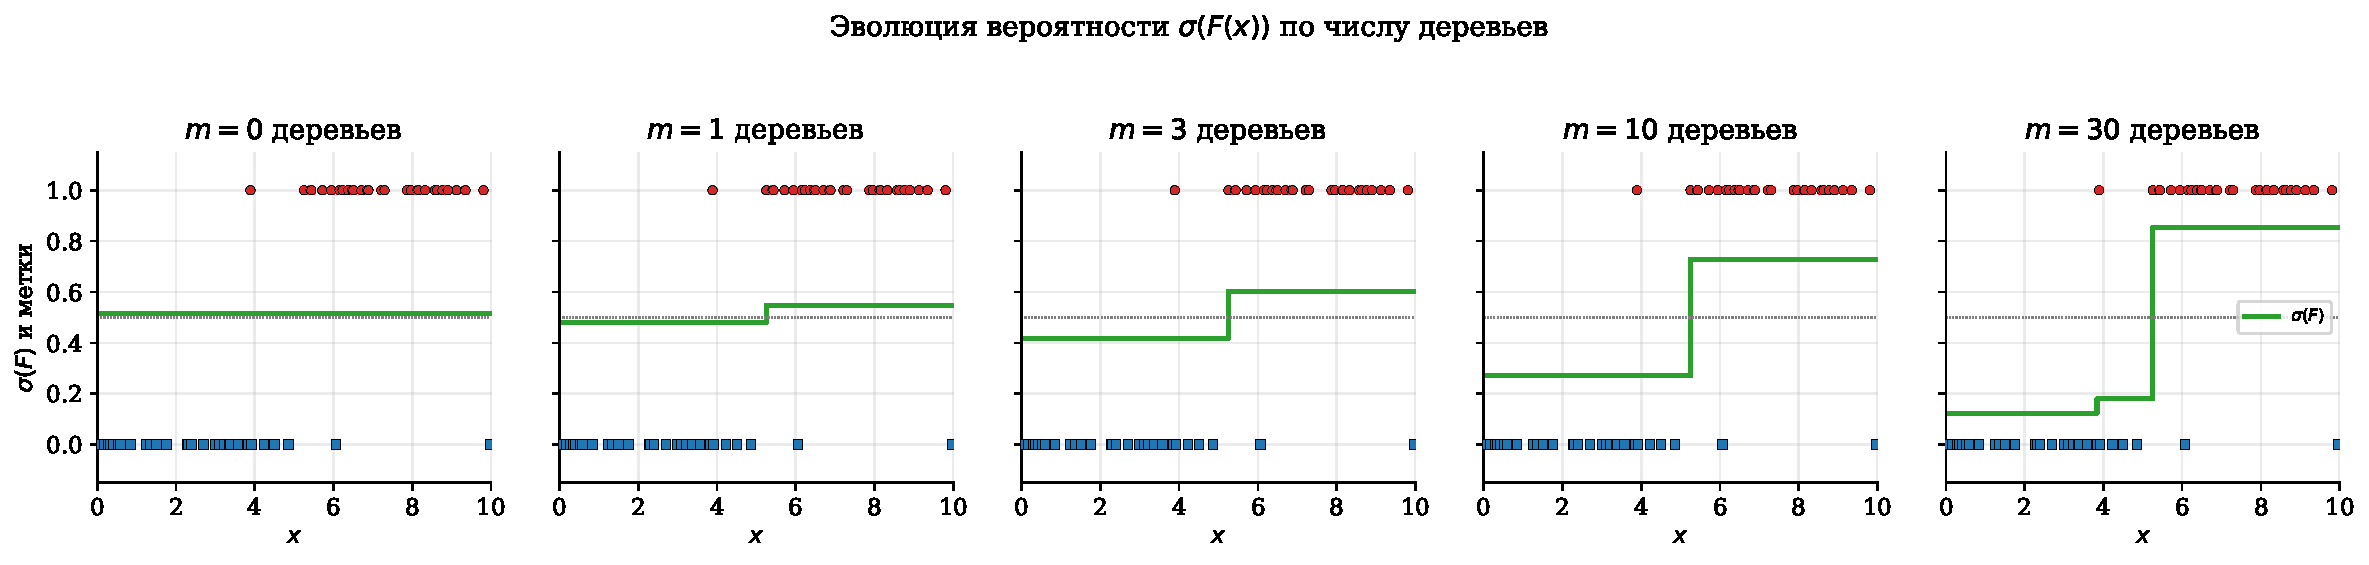
\includegraphics[width=1.0\linewidth]{boosting_evolution.pdf}
  \caption{Эволюция вероятности $\sigma(F(x))$ для одномерной задачи по мере добавления деревьев. На $m = 0$ модель плоская~--- одна константа $F_0$. С каждым добавленным stump'ом ступенька на границе становится круче и кривая лучше согласуется с метками. К $m = 30$ переход уже резкий и проходит близко к истинной границе.}
\end{figure}

% ==============================================================================
\section{One-vs-Rest для мультикласса}

\subsection{Идея}

У нас 6 классов активности (WALKING, ..., LAYING). Бустинг, который мы построили, бинарный. Как расширить?

Простейший способ~--- \textbf{One-vs-Rest}: для каждого класса $k = 1, \ldots, 6$ обучаем \emph{отдельный} бинарный классификатор $F^{(k)}$, который отличает «класс $k$» от «всех остальных». Получаем 6 моделей.

\textbf{Предсказание для нового $x$:}
\begin{enumerate}
  \item Для каждого $k$ считаем $\hat{p}_k^{\text{raw}}(x) = \sigma(F^{(k)}(x))$.
  \item Нормируем: $\displaystyle \hat{p}_k(x) = \frac{\hat{p}_k^{\text{raw}}}{\sum_{j=1}^K \hat{p}_j^{\text{raw}}}$.
  \item $\hat{y}(x) = \argmax_k \hat{p}_k(x)$.
\end{enumerate}

\subsection{Зачем нормировка}

Каждый бинарный $\sigma(F^{(k)})$~--- это вероятность класса $k$ против всех. Сумма по $k$ не обязана быть равна 1: каждый классификатор тренировался независимо. Нормировка делает $\hat{p}_k$ распределением вероятностей.

\begin{warning}
Это не математически корректное превращение в multinomial-вероятности (для этого нужен softmax по логитам, а не нормировка сигмоид). Но для argmax это эквивалентно: $\argmax_k \sigma(F^{(k)}) = \argmax_k \hat{p}_k$, потому что нормировка~--- умножение на одну и ту же константу для всех $k$.

Разница с честным multinomial-бустингом проявляется только в \emph{калибровке} вероятностей (насколько $\hat{p}_k$ совпадает с истинной частотой класса), но не в качестве классификации по argmax.
\end{warning}

\subsection{Альтернатива: multinomial softmax}

В «правильном» multi-class бустинге мы держим $K$ отдельных функций $F^{(1)}, \ldots, F^{(K)}$ и считаем
\[
  \Pr(y = k \mid x) = \frac{e^{F^{(k)}(x)}}{\sum_{j=1}^K e^{F^{(j)}(x)}}.
\]

Loss~--- кросс-энтропия. Residuals для класса $k$:
\[
  r_i^{(k)} = [y_i = k] - \frac{e^{F^{(k)}(x_i)}}{\sum_j e^{F^{(j)}(x_i)}}.
\]

И на каждой итерации обучаем $K$ деревьев (по одному на класс) на эти residuals. Так делает sklearn-овский \texttt{GradientBoostingClassifier} с \texttt{multinomial}-режимом.

Мы выбрали OvR ради простоты~--- наша реализация остаётся бинарной, обёртка вокруг неё тривиальна. Цена~--- классификаторы не «знают» друг о друге, и общая структура задачи теряется. На HAR разница в качестве небольшая, потому что классы относительно разнесены.

% ==============================================================================
\section{Метрики, матрица ошибок, ROC по классам}

\subsection{Многоклассовые версии метрик}

Те же accuracy/precision/recall/F1, но:
\begin{itemize}
  \item \textbf{Accuracy}~--- просто доля верных предсказаний:
    $\frac{1}{n}\sum_i [\hat{y}_i = y_i]$.
  \item \textbf{Precision/Recall/F1 для класса $k$} считаются как в бинарном случае с разбиением «класс $k$ vs остальные».
  \item \textbf{Macro-усреднение}~--- среднее по классам с равным весом: $\frac{1}{K}\sum_k \text{Precision}_k$.
  \item \textbf{Micro-усреднение}~--- суммируем TP/FP/FN по классам и считаем глобально. Для multiclass с одинаковым приоритетом классов micro accuracy = accuracy.
\end{itemize}

В отчёте используется macro, чтобы каждый класс вносил равный вклад, независимо от количества примеров.

\subsection{Матрица ошибок $K \times K$}

Строки~--- истинный класс, столбцы~--- предсказанный. Элемент $(i, j)$~--- число объектов класса $i$, предсказанных как $j$. Диагональ~--- правильные предсказания.

Из матрицы видны характерные ошибки: например, в HAR большая ячейка $(SITTING, STANDING) = 178$ означает, что 178 примеров SITTING были классифицированы как STANDING.

\subsection{ROC One-vs-Rest}

Для каждого класса $k$ строим бинарную задачу «класс $k$ vs все остальные» и считаем ROC-кривую этой задачи (по вероятностям $\hat{p}_k$). Получаем $K$ кривых.

AUC по классу $k$~--- площадь под кривой для этой бинарной задачи. AUC = 1 для LAYING означает: классификатор всегда ранжирует «лежать» выше всех других классов; есть порог, при котором все 537 LAYING-примеров классифицируются верно без ложных срабатываний.

\begin{intuition}
Высокий AUC при средних accuracy и F1 говорит, что модель \emph{хорошо ранжирует}, но при близких вероятностях двух соседних классов (SITTING vs STANDING) argmax иногда ошибается. AUC «не видит» этой ошибки, потому что считает ранжирование внутри одного класса против всех остальных, а argmax-конкуренция SITTING/STANDING~--- это «между собой».
\end{intuition}

% ==============================================================================
\section{Что важно запомнить}

\begin{itemize}
  \item \textbf{Бустинг}~--- последовательная сумма слабых учителей, где каждый следующий исправляет ошибки предыдущих в направлении отрицательного градиента loss.
  \item \textbf{Decision stump}~--- дерево глубины 1: одно правило «$x_j \le t$» и два листовых значения. Оптимальные листовые значения для MSE-задачи~--- средние остатков в листах.
  \item \textbf{Сигмоида $\sigma(F) = 1/(1+e^{-F})$}~--- обратная функция к log-odds, переводит сырой выход в вероятность.
  \item \textbf{Log-loss}~--- негатив логарифма правдоподобия Бернулли, штрафует уверенно-неверные ответы.
  \item \textbf{Ключевая формула:} $-\partial L/\partial F = y - \sigma(F)$. Получается из $\sigma'(F) = \sigma(F)(1 - \sigma(F))$.
  \item \textbf{Стартовое значение} $F_0 = \log(p/(1-p))$~--- оптимальная константа, минимизирующая log-loss без учёта $x$.
  \item \textbf{Learning rate $\nu$}~--- регуляризатор: маленький шаг → больше деревьев → лучшее обобщение.
  \item \textbf{Feature subsampling}~--- ускоряет обучение и снижает корреляцию между stump'ами.
  \item \textbf{OvR}~--- $K$ бинарных классификаторов плюс нормировка сигмоид. Простая обёртка, эквивалентная argmax с честным multinomial.
  \item \textbf{Высокий AUC + средний F1}~--- бустинг хорошо ранжирует, но argmax спотыкается, когда соседние классы дают близкие вероятности.
\end{itemize}

\end{document}
